\documentclass[11pt]{article}

\newcommand{\yourname}{Zerun Tian}
\newcommand{\yourcollaborators}{}

\def\comments{0}
\setlength{\parindent}{0 in}
\setlength{\parskip}{0.1in}


%format and packages

%\usepackage{algorithm, algorithmic}
\usepackage{algpseudocode}
\usepackage{amsmath, amssymb, amsthm}
\usepackage{enumerate}
\usepackage{enumitem}
\usepackage{framed}
\usepackage{verbatim}
\usepackage[margin=1.0in]{geometry}
\usepackage{microtype}
\usepackage{kpfonts}
\usepackage{graphicx}       % upload image
\usepackage{palatino}
	\DeclareMathAlphabet{\mathtt}{OT1}{cmtt}{m}{n}
	\SetMathAlphabet{\mathtt}{bold}{OT1}{cmtt}{bx}{n}
	\DeclareMathAlphabet{\mathsf}{OT1}{cmss}{m}{n}
	\SetMathAlphabet{\mathsf}{bold}{OT1}{cmss}{bx}{n}
	\renewcommand*\ttdefault{cmtt}
	\renewcommand*\sfdefault{cmss}
	\renewcommand{\baselinestretch}{1.06}
\usepackage[usenames,dvipsnames]{xcolor}
\definecolor{DarkGreen}{rgb}{0.15,0.5,0.15}
\definecolor{DarkRed}{rgb}{0.6,0.2,0.2}
\definecolor{DarkBlue}{rgb}{0.2,0.2,0.6}
\definecolor{DarkPurple}{rgb}{0.4,0.2,0.4}
\usepackage[pdftex]{hyperref}
\hypersetup{
	linktocpage=true,
	colorlinks=true,				% false: boxed links; true: colored links
	linkcolor=DarkBlue,		% color of internal links
	citecolor=DarkBlue,	% color of links to bibliography
	urlcolor=DarkBlue,		% color of external links
}

%enclosure macros
\newcommand{\paren}[1]{\ensuremath{\left( {#1} \right)}}
\newcommand{\bracket}[1]{\ensuremath{\left\{ {#1} \right\}}}
\renewcommand{\sb}[1]{\ensuremath{\left[ {#1} \right\]}}
\newcommand{\ab}[1]{\ensuremath{\left\langle {#1} \right\rangle}}

%probability macros
\newcommand{\ex}[2]{{\ifx&#1& \mathbb{E} \else \underset{#1}{\mathbb{E}} \fi \left[#2\right]}}
\newcommand{\pr}[2]{{\ifx&#1& \mathbb{P} \else \underset{#1}{\mathbb{P}} \fi \left[#2\right]}}
\newcommand{\var}[2]{{\ifx&#1& \mathrm{Var} \else \underset{#1}{\mathrm{Var}} \fi \left[#2\right]}}

%useful CS macros
\newcommand{\poly}{\mathrm{poly}}
\newcommand{\polylog}{\mathrm{polylog}}
\newcommand{\zo}{\{0,1\}}
\newcommand{\pmo}{\{\pm1\}}
\newcommand{\getsr}{\gets_{\mbox{\tiny R}}}
\newcommand{\card}[1]{\left| #1 \right|}
\newcommand{\set}[1]{\left\{#1\right\}}
\newcommand{\negl}{\mathrm{negl}}
\newcommand{\eps}{\varepsilon}
\DeclareMathOperator*{\argmin}{arg\,min}
\DeclareMathOperator*{\argmax}{arg\,max}
\newcommand{\eqand}{\qquad \textrm{and} \qquad}
\newcommand{\ind}[1]{\mathbb{I}\{#1\}}
\newcommand{\sslash}{\ensuremath{\mathbin{/\mkern-3mu/}}}

%mathbb
\newcommand{\N}{\mathbb{N}}
\newcommand{\R}{\mathbb{R}}
\newcommand{\Z}{\mathbb{Z}}
%mathcal
\newcommand{\cA}{\mathcal{A}}
\newcommand{\cB}{\mathcal{B}}
\newcommand{\cC}{\mathcal{C}}
\newcommand{\cD}{\mathcal{D}}
\newcommand{\cE}{\mathcal{E}}
\newcommand{\cF}{\mathcal{F}}
\newcommand{\cL}{\mathcal{L}}
\newcommand{\cM}{\mathcal{M}}
\newcommand{\cO}{\mathcal{O}}
\newcommand{\cP}{\mathcal{P}}
\newcommand{\cQ}{\mathcal{Q}}
\newcommand{\cR}{\mathcal{R}}
\newcommand{\cS}{\mathcal{S}}
\newcommand{\cU}{\mathcal{U}}
\newcommand{\cV}{\mathcal{V}}
\newcommand{\cW}{\mathcal{W}}
\newcommand{\cX}{\mathcal{X}}
\newcommand{\cY}{\mathcal{Y}}
\newcommand{\cZ}{\mathcal{Z}}

%theorem macros
\newtheorem{thm}{Theorem}
\newtheorem{lem}[thm]{Lemma}
\newtheorem{fact}[thm]{Fact}
\newtheorem{clm}[thm]{Claim}
\newtheorem{rem}[thm]{Remark}
\newtheorem{coro}[thm]{Corollary}
\newtheorem{prop}[thm]{Proposition}
\newtheorem{conj}[thm]{Conjecture}

\theoremstyle{definition}
\newtheorem{defn}[thm]{Definition}


\newcommand{\instructor}{Virgil Pavlu}
\newcommand{\hwnum}{9}
\newcommand{\hwdue}{Wednesday, May 20 at 11:59pm via \href{https://gradescope.com/courses/229309}{Gradescope}}

\theoremstyle{theorem}
\newtheorem{prob}{}
\newtheorem{sol}{Solution}

\definecolor{cit}{rgb}{0.05,0.2,0.45} 
\newcommand{\solution}{\medskip\noindent{\color{DarkBlue}\textbf{Solution:}}}

\begin{document}
{\Large 
\begin{center}{CS5800: Algorithms} --- Spring '21 --- \instructor \end{center}}
{\large
\vspace{10pt}
\noindent Homework~\hwnum \vspace{2pt}\\
Submit via \href{https://www.gradescope.com/courses/232127}{Gradescope}}

\bigskip
{\large \noindent Name: \yourname }

{\large \noindent Collaborators: \yourcollaborators}

\vspace{15pt}

{\large \noindent Instructions:}

\begin{itemize}

\item Make sure to put your name on the first page.  If you are using the \LaTeX~template we provided, then you can make sure it appears by filling in the \texttt{yourname} command.

\item Please review the grading policy outlined in the course information page.

\item You must also write down with whom you worked on the assignment.  If this changes from problem to problem, then you should write down this information separately with each problem.

\item Problem numbers (like Exercise 3.1-1) are corresponding to CLRS $3^{rd}$ edition.  While the  $2^{nd}$ edition  has  similar  problems  with  similar  numbers,  the  actual  exercises  and their solutions are different, so make sure you are using the $3^{rd}$ edition.

\end{itemize}

%%% Problem 1 %%%
\newpage
\begin{prob} \textbf{(25 points)} Exercise 17.3-3.(Hint:  a reasonable potential function to use is $\phi(D_i) =kn_i$· $\ln n_i$ where $n_i$ is the number of elements in the binary heap,  and $k$ is a big enough constant.  You can use this function and just show the change in potential for each of the two operations.)
\end{prob}

Consider an ordinary binary min-heap data structure with $n$ elements supporting the instructions $\textproc{\textsc{Insert}}$ and $\textproc{\textsc{Extract-Min}}$ in $O(\lg n)$ worst-case time. Give a potential function $\phi$ such that the amortized cost of $\textproc{\textsc{Insert}}$ is $O(\lg n)$ and the amortized cost of $\textproc{\textsc{Extract-Min}}$ is $O(1)$, and show that it works.

\solution

Using the given potential function, we find that $\phi(D_0) = 0$ when the heap is empty. Then, for all $i > 0$, $n_i$ will never drop 0, so $\phi(D_i) \ge 0 = \phi(D_0)$. Therefore, the total amortized cost of a sequence of $n$ operations is an upper bound on the total actual cost.

Let's first evaluate an expression $n \cdot \ln (n/(n-1))$ which will help simplifying derivations below. 
\[
\begin{split}
\lim_{n \to \infty} n \cdot \frac{n}{n-1} = \lim_{n \to \infty} \ln \left[ (\frac{n}{n-1})^n \right] &= \lim_{n \to \infty} \ln \left[ (\frac{n-1+1}{n-1})^n \right] \\
&= \lim_{n \to \infty} \ln \left[ (1 + \frac{1}{n-1})^n \right] \\
&= \lim_{n \to \infty} \ln \left[ \left( (1 + \frac{1}{n-1})^{n-1} \right)^{\frac{n}{n-1}}  \right] \\
&= \lim_{n \to \infty} \ln \left[ \left( e \right)^{\frac{n}{n-1}}  \right] \\
&= \lim_{n \to \infty} \frac{n}{n-1} \\
&= 1
\end{split}
\]
Note that $\lim_{n \to \infty} (1 + 1/x)^{x} = e$.

Suppose the $i$-th operation is $\textproc{\textsc{Insert}}$, its amortized cost is,
\[
\begin{split}
\hat{c}_i &= c_i + \phi(D_i) - \phi(D_{i-1}) \\
& \le k \cdot \ln n_i +  k n_i \cdot \ln n_i - k (n_i - 1) \cdot \ln (n_i - 1) \\
& = k \cdot \ln n_i +  k n_i \cdot \ln n_i - k n_i \cdot \ln (n_i - 1) + k \cdot \ln (n_i - 1) \\
& \le 2k \cdot \ln n_i  + k n_i \cdot (\ln n_i - \ln (n_i - 1)) \\
& = 2k \cdot \ln n_i  + k n_i \cdot \ln \frac{n_i}{(n_i - 1)} \\
& \le 2k \cdot \ln n_i  + k \cdot c \text{ (based on the trick above) } \\
& = O(\lg n_i)
\end{split}
\]
Note that $n_{i-1} = n_i - 1$ because we had one less element before the insertion.

Suppose the $i$-th operation is $\textproc{\textsc{Extract-Min}}$, its amortized cost is,
\[
\begin{split}
\hat{c}_i &= c_i + \phi(D_i) - \phi(D_{i-1}) \\
& = k \cdot \ln n_i + k n_i \cdot \ln n_i - k n_{i-1} \cdot \ln n_{i-1} \\
& \le k \cdot \ln n_{i-1} + k (n_{i-1} - 1) \cdot \ln (n_{i-1} - 1) - k n_{i-1} \cdot \ln n_{i-1} \\
& = k \cdot \ln n_{i-1} + k n_{i-1} \cdot \ln (n_{i-1} - 1)  - k \cdot \ln (n_{i-1} - 1) - k n_{i-1} \cdot \ln n_{i-1} \\
& = k \cdot (\ln n_{i-1} - \ln (n_{i-1} - 1)) + k n_{i-1} \cdot (\ln (n_{i-1} - 1) - \ln n_{i-1}) \\
& = k \cdot \ln \frac{n_{i-1}}{n_{i-1} - 1} + k n_{i-1} \cdot \ln \frac{n_{i-1} - 1}{n_{i-1}} \\
& \le k \cdot c + k n_{i-1} \cdot \ln (\frac{n_{i-1}}{n_{i-1}-1})^{-1} \\
& \le k \cdot c - k \cdot c' \text{ (based on the trick above) } \\
& = k \cdot c - k \cdot c' \\
& = O(1)
\end{split}
\]

Note that $n_i = n_{i-1} - 1$ because we had one more element before extracting the min.

The given potential function lets us derive that the amortized cost of $\textproc{\textsc{Insert}}$ is $O(\lg n)$ and the amortized cost of $\textproc{\textsc{Extract-Min}}$ is $O(1)$.


%%% Problem 2 %%%
\newpage
\begin{prob} \textbf{(25 points)} Exercise 17.3-6.
\end{prob}
Show how to implement a queue with two ordinary stacks (Exercise 10.1-6) so that the amortized cost of each $\textproc{\textsc{Enqueue}}$ and each $\textproc{\textsc{Dequeue}}$ operation is $O(1)$.

\solution

We have implemented such a queue in hw7-8. Here is the pseudocode for $\textproc{\textsc{Enqueue}}$ and $\textproc{\textsc{Dequeue}}$.

\begin{algorithmic}[1]
\Function{Enqueue}{$A$, $B$, $x$}
	\State $\textproc{\textsc{Push}}(A, x)$ \Comment{call the $\textproc{\textsc{Push}}$ api of stack}
\EndFunction
\end{algorithmic}

$\textproc{\textsc{Enqueue}}$'s implementation is trivial. Dequeuing an element involves first checking if the stack $B$ has any elements. If it does, we don't move things around; otherwise, we transfer every element from $A$ to $B$. Eventually, we pop the top element of $B$.

\begin{algorithmic}[1]
\Function{Dequeue}{$A$, $B$}
	\If {\textproc{\textsc{Stack-Empty}}(B)}
		\While {\textbf{not} \textproc{\textsc{Stack-Empty}}(A)}
			\State $x = \textproc{\textsc{Pop}}(A)$
			\State $\textproc{\textsc{Push}}(B, x)$
		\EndWhile
	\EndIf
	\State $\textbf{return } \textproc{\textsc{Pop}}(B)$
\EndFunction
\end{algorithmic}

The actual cost of $\textproc{\textsc{Enqueue}}$ is 1 and the cost of $\textproc{\textsc{Dequeue}}$ depends on whether stack $B$ is empty. In the best case, i.e. $B$ is not empty, the cost is 1. In the worst case, i.e. $B$ is empty, the cost is two times $k$, the number of elements in $A$, plus 1.

We define the following amortized costs: $\textproc{\textsc{Enqueue}}$ operation costs 4; $\textproc{\textsc{Dequeue}}$ operation costs 0.

We can pay for any sequence of queue operations by charging the amortized costs. Here is how. When we enqueue, we push an element onto the stack $A$. We spend 1 for the actual cost and save 3 credits for later. Consequently, every element of $A$ owns 3 credits that can be used by subsequent operations. For any element to be dequeued, it has to go through the process of being popped out from $A$, then being pushed onto $B$, and finally being popped from $B$. Each of the three phases costs exactly 1 credit, which has been prepaid when the element is enqueued. Thus, we have always charged enough up front to pay for $\textproc{\textsc{Dequeue}}$ operations. This implies that the total amortized cost is an upper bound on the total actual cost. 

Hence, we showed that the amortized cost of every operation could be $O(1)$ in such design.


%%% Problem 3 %%%
\newpage
\begin{prob} \textbf{(25 points)} Exercise 19.2-1.
\end{prob}

Show the Fibonacci heap that results from calling $\textproc{\textsc{Fib-Heap-Extract-Min}}$ on the Fibonacci heap shown in Figure 19.4(m).

\solution

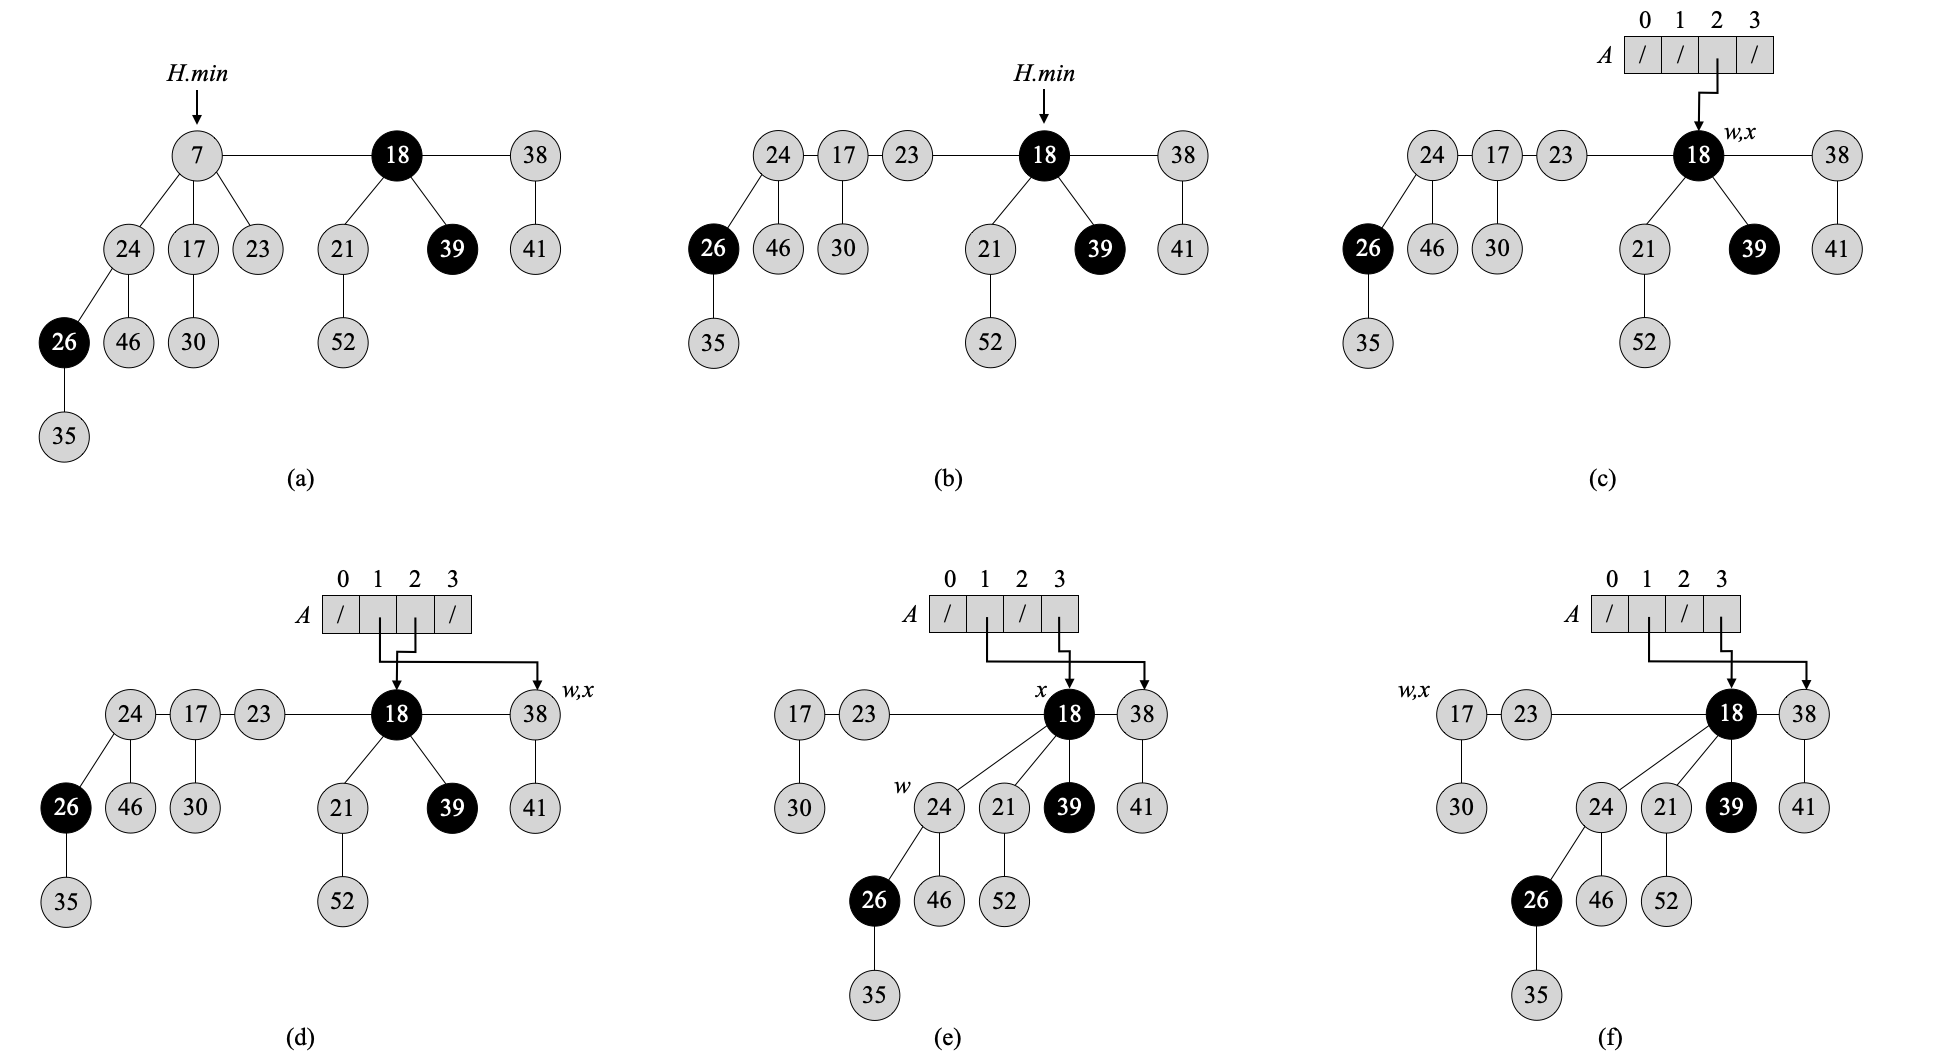
\includegraphics[scale=0.5]{./hw9q3-1.png}

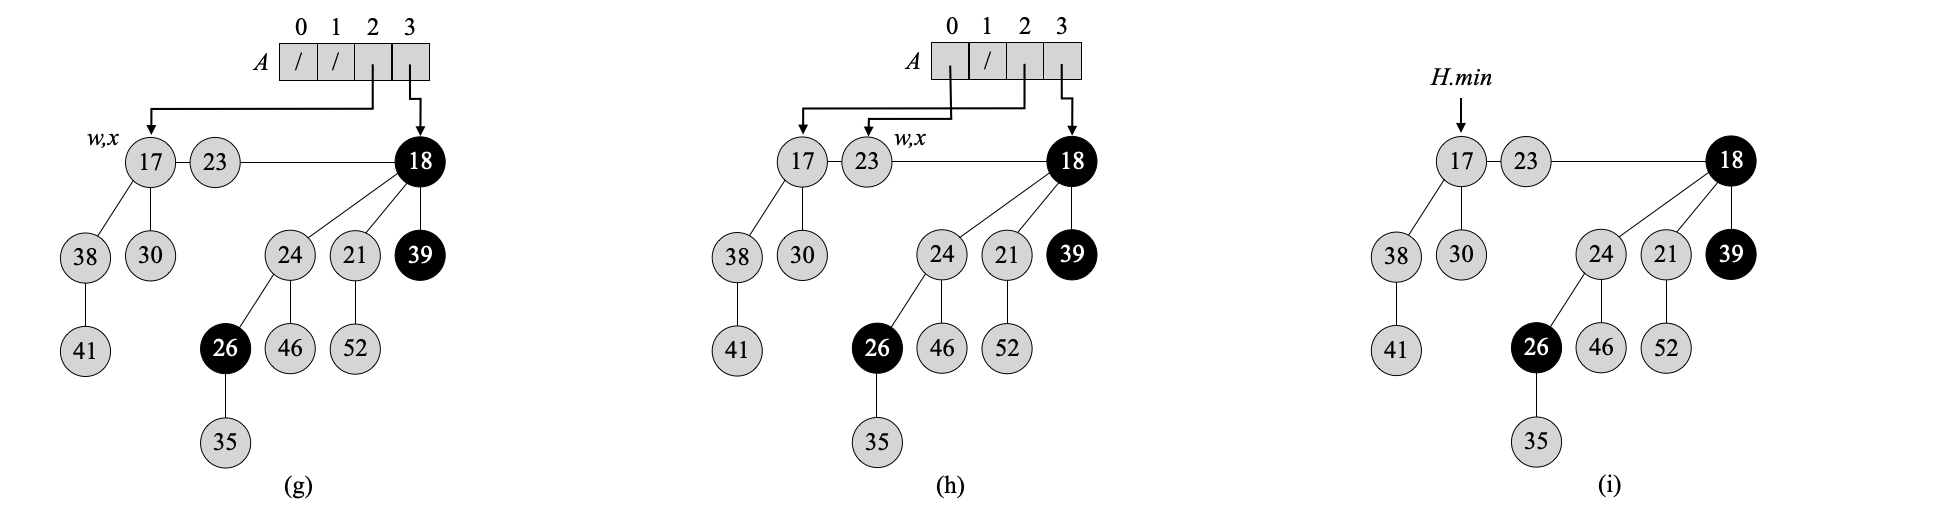
\includegraphics[scale=0.5]{./hw9q3-2.png}

In (a), we show the 19.4(m) setup. In (b), we remove the current min 7, meld its children into the root list, and move the min pointer to its right child. In (c), we start to run the $\textproc{\textsc{Consolidate}}$ procedure. An array $A$ is initialized to keep track of root nodes of different degrees for the purpose of merging. In (e), we are handling the node with value 24 whose degree is 2. Because the array $A$ has tracked another root node with degree 2, a merge operation is performed, which results in the configuration (e). The next node to be processed is the node with value 17. It has degree 1 which is consistent with the degree of node 38 according to $A$. The resulting configuration is shown in (g). Last but not the least, the node with value 23 has degree 0 which is the only root node of that degree. Finally, we construct $H$ with nodes linked in $A$ and update the min pointer.



%%% Problem 4 %%%
\newpage
\begin{prob} \textbf{(50 points)} Implement  binomial  heaps  as  described  in  class  and  in  the  book.   You should use links (pointers) to implement the structure as shown in the fig~\ref{fig:binomialheaps}.  

Your implementation should include the operations:  Make-heap, Insert, Minimum, Extract-Min, Union, Decrease-Key, Delete
\end{prob}

\begin{figure}[!ht]
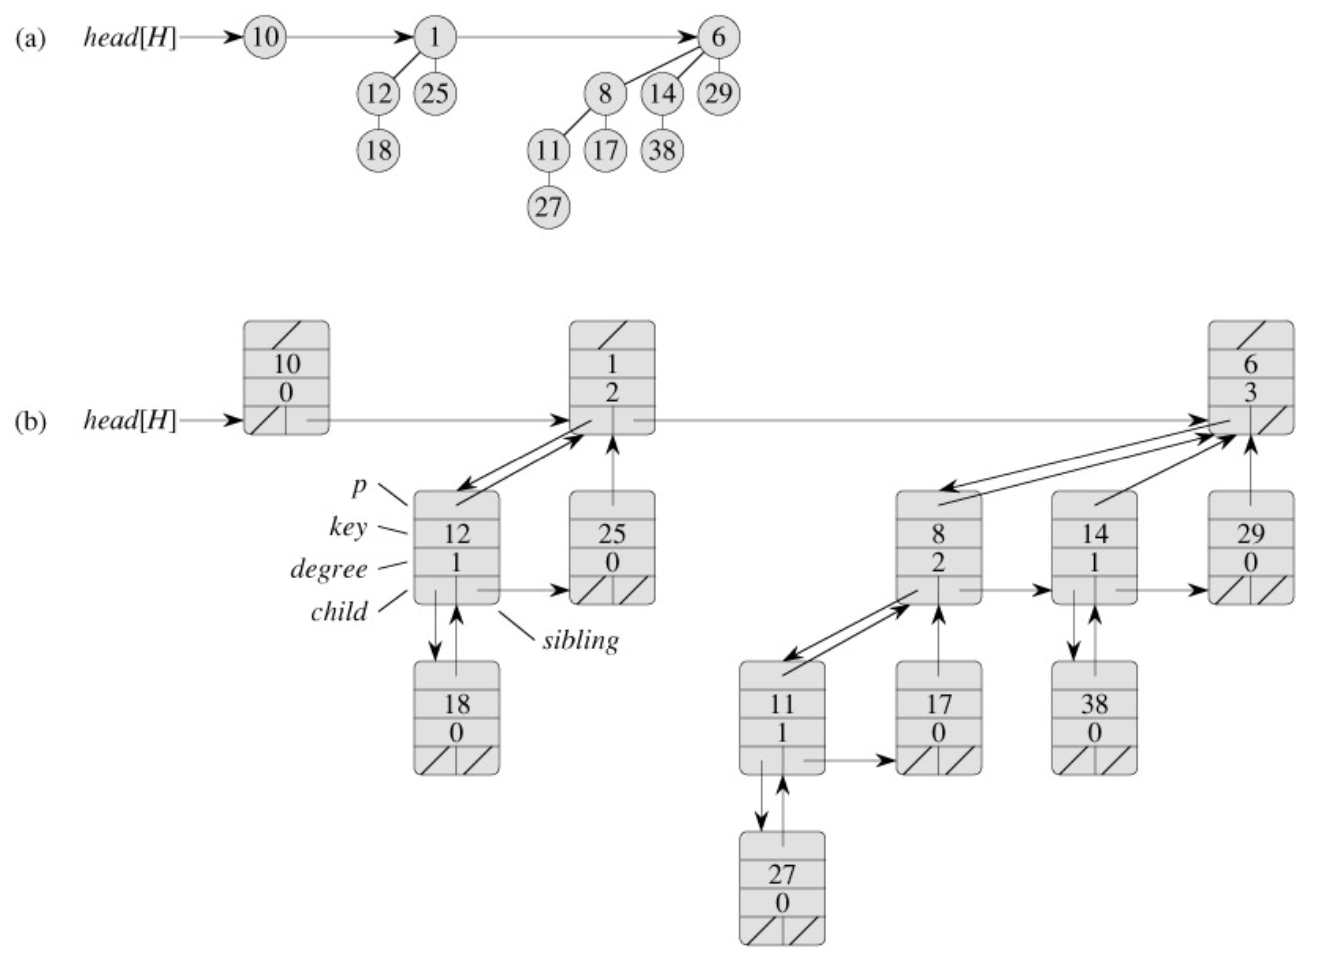
\includegraphics[width=15cm]{./hw9_fig1.png}
\caption{Binomial Heaps}
\label{fig:binomialheaps}
\end{figure}

\noindent Make  sure  to  preserve  the  characteristics  of  binomial  heaps  at  all  times:

\begin{enumerate}
\item (1) each component should be a binomial tree with children-keys bigger than the parent-key;

\item (2)  the  binomial  trees  should  be  in  order  of  size  from  left  to  right.   Test  your  code several arrays set of random generated integers (keys).
\end{enumerate}

\solution

Code is listed in the next few pages.


%%% Problem 5 (EC) %%%
\newpage
\begin{prob} \textbf{(Extra Credit)} Find a way to nicely draw the binomial heap created from input, like in the figure.
\end{prob}
\solution

%%% Problem 6 (EC) %%%
\begin{prob} \textbf{(Extra Credit)} Write code to implement Fibonacci Heaps, with discussed operations:ExtractMin, Union, Consolidate, DecreaseKey, Delete.
\end{prob}
\solution

%%% Problem 7 (EC) %%%
\begin{prob} \textbf{(Extra Credit)} Figure out what are the marked nodes on Fibonacci Heaps.  In particular explain how the potential function works for FIB-HEAP-EXTRACT-MEAN and FIB-HEAP-DECREASE-KEY operations.
\end{prob}
\solution

\end{document}